\documentclass[11pt]{article}

\usepackage[margin=1in]{geometry}
\usepackage{booktabs}
\usepackage{array}
\usepackage{graphicx}
\usepackage{float}
\usepackage{longtable}
\usepackage{xcolor}
\usepackage{enumitem}
\usepackage{hyperref}
\usepackage{fancyvrb}
\usepackage{tcolorbox}

\hypersetup{colorlinks=true, linkcolor=blue!50!black, urlcolor=blue!50!black}

\newcommand{\code}[1]{\texttt{#1}}

\title{\textbf{Live Benchmark Report\\Cost-Optimizing LLM Router}}
\author{Systems for Machine Learning --- Final Project}
\date{}

\begin{document}
\maketitle

\noindent\textbf{Runs:} \code{tpu\_bench\_001} (2026-06-10, 46 problems) $\cdot$
\code{tpu\_bench\_002} (2026-06-11, 88 problems)\\
\textbf{Combined sample:} 134 problems attempted across 4 domains (math, reasoning,
factual, code).

\vspace{0.5em}
\noindent These are \textbf{live} end-to-end runs (real router model on a TPU + real
external solver calls through OpenRouter), not the mocked smoke test. They exercise
the full path:

\begin{tcolorbox}[colback=gray!8,colframe=gray!40,boxrule=0.4pt]
\small\ttfamily
problem $\rightarrow$ local router (TPU) $\rightarrow$ 2-pass model pick $\rightarrow$
resolution server $\rightarrow$ OpenRouter solver $\rightarrow$ validation
$\rightarrow$ cost $\rightarrow$ metrics
\end{tcolorbox}

\section*{Infrastructure}

\begin{longtable}{@{}>{\raggedright}p{0.26\textwidth} p{0.66\textwidth}@{}}
\toprule
\textbf{Component} & \textbf{Detail} \\
\midrule
Host & Google Cloud TPU VM \code{lab-2} (\code{v5litepod-1} / TPU v5e, 16\,GB HBM) \\
Router model & \code{ibm-granite/granite-4.1-3b} served by vLLM on the TPU (\code{:7654}, bf16) \\
Resolution server & FastAPI \code{/solve} (\code{:8001}) \\
Solver provider & OpenRouter (free tier) \\
Routable lineup & \code{gpt-oss-20b} (21B/3.6B) $\cdot$ \code{gpt-oss-120b} (117B/5.1B) $\cdot$ \code{qwen3-coder} (480B/35B) $\cdot$ \code{nemotron-3-ultra-550b-a55b} (550B/55B, escalation target) \\
Driver & \code{local-inference/main.py} \\
\bottomrule
\end{longtable}

\section*{Methodology}

\begin{itemize}[leftmargin=1.4em]
\item \textbf{Routing:} the local granite model makes a 2-pass decision per problem
  (pick a model, then self-revise) and emits JSON \code{\{model\_id, reasoning\}}.
\item \textbf{Validation:} \code{math} via \code{numeric\_match} heuristic,
  \code{reasoning} via curated validators, \code{code} via \code{verify: tests}
  (candidate run against its asserts in a sandbox, with a solve$\rightarrow$run$\rightarrow$repair
  loop on failure).
\item \textbf{Cost:} the project's custom cost function (params + tokens), not provider
  prices. Accumulated per problem by \code{CostAccumulator}.
\end{itemize}

\section*{How the router decides which model to forward to}

Routing is performed \textbf{on-device} by the small \code{granite-4.1-3b} model (vLLM
on the TPU); the larger solver models are never consulted for the decision. The policy
is prompt-driven and implemented in \code{local-inference/utils.py}
(\code{LogicManager} / \code{LocalInferenceManager}). Per problem:

\begin{enumerate}[leftmargin=1.6em]
\item \textbf{Build the routing prompt} (\code{\_init\_routing\_prompt}). A system
  prompt is assembled from \code{configs/prompts.yaml} plus a rendered ``menu'' of
  every candidate model from \code{configs/models.yaml} --- each line carries the model
  id, \textbf{total / active parameters}, and a one-line \textbf{capability
  description} (e.g.\ ``performs like a high-schooler'' vs ``PhD-student level
  reasoning''). The instruction is explicitly cost-minimizing:
  \begin{quote}\itshape
  ``You are a router with the goal of minimizing cost. Given a problem, pick the least
  expensive model that is likely to solve it correctly. Use the model descriptions and
  problem difficulty to avoid both over-routing and under-routing \ldots Also ask
  whether a student at the level described in the model description could solve this
  problem.''
  \end{quote}
  The router must emit \textbf{strict JSON}:
  \code{\{"reasoning": "...", "model\_id": "provider/model:free"\}}. (An optional
  \code{capabilities} prompt mode also injects per-model benchmark scores from
  \code{configs/benchmarks.yaml}.)

\item \textbf{Local short-circuit} (\code{\_can\_solve\_locally}). If
  \code{--local-model-solves} is on \textbf{and} the problem is
  \code{difficulty=very\_easy}, \code{verify=match}, and ships a reference answer, it is
  answered locally (\code{model\_id="local-router"}) with \textbf{no external call} ---
  the cheapest possible path.

\item \textbf{Two-pass decision} (\code{call\_model}, \code{temperature=0}, output
  capped at \code{ROUTER\_MAX\_OUTPUT\_TOKENS=2048}):
  \begin{itemize}[leftmargin=1.4em]
  \item \textbf{Pass 1 --- pick:} system = routing prompt, user = problem text $\rightarrow$
    the model emits \code{\{reasoning, model\_id\}}.
  \item \textbf{Pass 2 --- self-critique:} the pass-1 JSON is appended as the assistant
    turn, then a fixed follow-up asks it to reconsider --- ``Look at your own logic. Do
    you believe a student of the level described is capable of this? \ldots revise your
    reasoning and model\_id if you believe you have made a mistake.'' The model emits a
    revised decision. \textbf{The revised \code{model\_id} is the one used.}
  \end{itemize}

\item \textbf{Parse \& normalize} (\code{parse\_router\_response},
  \code{\_normalize\_model\_id}). The first \code{\{...\}} object is extracted (tolerant
  of single-quoted JSON). The chosen \code{model\_id} is checked against the set of
  valid ids from \code{models.yaml}; if it is missing or unrecognized, the router
  \textbf{falls back to the strongest model} (\code{nemotron-3-ultra-550b}) so an
  unparseable decision fails safe rather than dropping the problem.

\item \textbf{Dispatch} (\code{\_build\_solve\_payload}). The run id, problem fields,
  selected \code{model\_id}, the router's \code{reasoning}, and \code{max\_attempts}
  (default 2) are POSTed to the resolution server's \code{/solve}. The server owns
  solving, validation, retries, and \textbf{escalation} within the attempt budget
  (surfaced as the \code{escalated} flag).
\end{enumerate}

\noindent\textbf{In effect} the decision is ``cheapest model whose described capability
level still covers this problem's difficulty,'' double-checked by a self-critique pass,
with a fail-safe to the strongest model. On this easy/medium sample that logic resolved
to \code{gpt-oss-20b} for every problem (see \emph{Routing behavior}); the
fallback-to-strongest path is what produced the \code{nemotron-550b} attempts on the
rate-limited calls.

\section*{Combined results (both runs)}

\begin{longtable}{@{}>{\raggedright}p{0.42\textwidth} p{0.5\textwidth}@{}}
\toprule
\textbf{Metric} & \textbf{Value} \\
\midrule
Problems attempted & 134 \\
Reached a solver & 133 \\
\textbf{Solved} & \textbf{120 / 133 (90.2\%)} \\
Solved, excluding rate-limited failures & \textbf{120 / 120 (100\%)} \\
Escalations & 0 \\
Failures & 13 $\times$ OpenRouter free-tier 429 + 1 dropped (router non-JSON) \\
Cost per solved problem & $\sim$\$9.8e-6 (custom units) \\
Routing & every reached problem $\rightarrow$ \code{openai/gpt-oss-20b:free} (cheapest tier) \\
\bottomrule
\end{longtable}

\section*{Router vs. each model individually}

The router's value proposition is \textbf{matching solve quality at the lowest cost}.
To show this we take the \textbf{133 served problems} and ask: what would it cost to
run the \emph{same workload} (identical observed prompt/completion tokens, per problem)
on each candidate model individually? Cost is computed with the project's own cost
function (\code{server/cost/cost\_function.py}); solve rate is the router's empirical
result.

\begin{figure}[H]
\centering
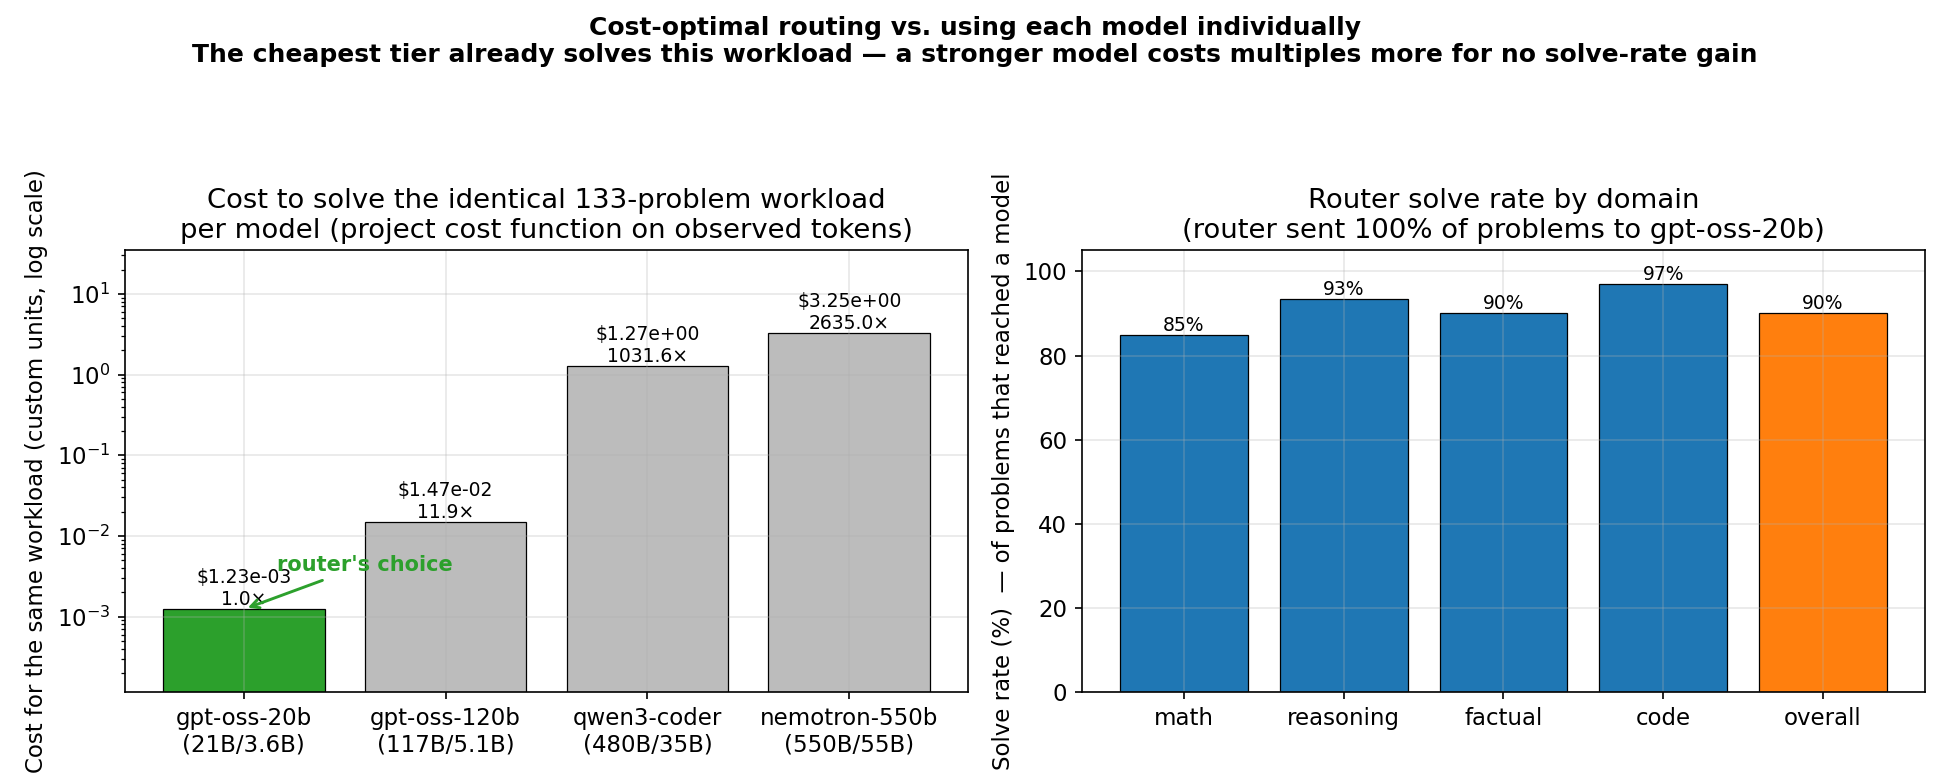
\includegraphics[width=\textwidth]{figures/router_vs_models.png}
\caption{Left: cost to serve the identical 133-problem workload under each model
(log scale), computed by the project cost function on the observed tokens. Right: the
router's empirical solve rate by domain --- it sent 100\% of problems to the cheapest
tier and still solved 90\% of problems that reached a model.}
\end{figure}

\begin{longtable}{@{}l r r@{}}
\toprule
\textbf{Strategy} & \textbf{Cost (same 133-problem workload)} & \textbf{vs. cheapest} \\
\midrule
\textbf{Router $\rightarrow$ gpt-oss-20b} (what it chose) & \textbf{\$0.001234} & \textbf{1.0$\times$} \\
Always gpt-oss-120b           & \$0.014700 & 11.9$\times$ \\
Always qwen3-coder (480B)     & \$1.272608 & 1{,}031.6$\times$ \\
Always nemotron-550b (550B)   & \$3.250420 & 2{,}635.0$\times$ \\
\bottomrule
\end{longtable}

\begin{itemize}[leftmargin=1.4em]
\item The router sent \textbf{100\%} of problems to the cheapest tier and still solved
  \textbf{90\% of problems that reached a model} (100\% excluding free-tier 429s).
  Using the strongest model (\code{nemotron-550b}) individually on the identical
  workload would cost \textbf{${\sim}2{,}635\times$} more --- for \textbf{no solve-rate
  headroom to gain}, since the cheapest model already solves this difficulty mix.
\item The modeled costs above are exact for the observed tokens; the \textbf{empirical}
  solve rates of the larger models on these same problems are a pending run (blocked on
  the OpenRouter free-tier daily cap; see Caveats).
\end{itemize}

\section*{Run 2 --- broader sample (\code{tpu\_bench\_002})}

Run after the daily free-tier cap reset; widened to 4 domains and ${\sim}2\times$ the
problems. Driver: \code{local-inference/main.py}, \code{--max-active 3}.

\subsection*{Overall}

\begin{longtable}{@{}>{\raggedright}p{0.42\textwidth} p{0.5\textwidth}@{}}
\toprule
\textbf{Metric} & \textbf{Value} \\
\midrule
Problems attempted / reached solver & 88 / 88 \\
\textbf{Solved} & \textbf{80 / 88 (90.9\%)} \\
Solved, excluding rate-limited failures & \textbf{80 / 80 (100\%)} \\
Escalations & 0 \\
Failures & 8 $\times$ OpenRouter free-tier 429 (no router-parse drops this run) \\
Total cost (custom units) & \$0.000790 \\
Cost per solved problem & $\sim$\$0.0000099 \\
Prompt / completion tokens & 13{,}405 / 8{,}060 \\
\bottomrule
\end{longtable}

\subsection*{By domain}

\begin{longtable}{@{}l r r r r r r@{}}
\toprule
\textbf{Domain} & \textbf{n} & \textbf{Solved} & \textbf{Solve rate} & \textbf{Esc.} & \textbf{Rate-limited} & \textbf{Cost} \\
\midrule
math      & 40 & 35 & 87.5\% & 0 & 5 & \$0.000318 \\
reasoning & 15 & 14 & 93.3\% & 0 & 1 & \$0.000105 \\
factual   & 10 &  9 & 90.0\% & 0 & 1 & \$0.000061 \\
code      & 23 & 22 & 95.7\% & 0 & 1 & \$0.000306 \\
\bottomrule
\end{longtable}

\begin{quote}
Same pattern as run 1: every problem the router reached went to
\code{openai/gpt-oss-20b:free} and solved first-try; \textbf{0 escalations},
\textbf{0 over-routing}. The only non-solves were 8 $\times$ OpenRouter 429 once the
free-tier daily cap was hit again. On the 429'd calls the driver fell back to the
configured \code{nemotron-3-ultra-550b} target (which also 429'd) --- the same
fallback path seen in run 1, not a capability escalation.
\end{quote}

\section*{Run 1 results (\code{tpu\_bench\_001})}

\begin{longtable}{@{}>{\raggedright}p{0.42\textwidth} p{0.5\textwidth}@{}}
\toprule
\textbf{Metric} & \textbf{Value} \\
\midrule
Problems attempted & 46 \\
Reached a solver & 45 \\
\textbf{Solved} & \textbf{40 / 45 (88.9\%)} \\
Solved, excluding rate-limited failures & \textbf{40 / 40 (100\%)} \\
Escalations & 0 \\
Failures & 5 (all OpenRouter free-tier rate-limit) + 1 dropped (router non-JSON) \\
Total cost (custom units) & \$0.000386 \\
Cost per solved problem & $\sim$\$0.0000096 \\
Prompt tokens & 6{,}586 \\
Completion tokens & 4{,}563 \\
Total solver attempts & 45 \\
\bottomrule
\end{longtable}

\subsection*{Results by domain}

\begin{longtable}{@{}l r r r r r r r r@{}}
\toprule
\textbf{Domain} & \textbf{n} & \textbf{Solved} & \textbf{Rate} & \textbf{Esc.} & \textbf{RL} & \textbf{Cost} & \textbf{P.tok} & \textbf{C.tok} \\
\midrule
math      & 20 & 16 & 80.0\%  & 0 & 4 & \$0.000138 & 2{,}493 & 1{,}248 \\
reasoning & 15 & 14 & 93.3\%  & 0 & 1 & \$0.000105 & 1{,}776 & 1{,}070 \\
code      & 10 & 10 & 100.0\% & 0 & 0 & \$0.000143 & 2{,}317 & 2{,}245 \\
\bottomrule
\end{longtable}

\begin{quote}
Every non-rate-limited problem in all three domains solved on the \textbf{first
attempt} (attempts = n per domain; no repair retries or escalations were triggered).
Code carried the most completion tokens per problem, as expected for generated
solutions.
\end{quote}

\section*{Routing behavior}

\begin{itemize}[leftmargin=1.4em]
\item For every successfully-routed problem, the granite router selected
  \code{openai/gpt-oss-20b:free} --- appropriate for this sample, which skews
  easy/medium (GSM8K-style word problems, short logic puzzles, and HumanEval-style
  functions the cheapest tier handles).
\item \textbf{0 escalations} and \textbf{0 over-routing} to the expensive tiers: no
  easy problem was sent to \code{qwen3-coder} or \code{nemotron}, and nothing that the
  small model solved needed the strongest model. On this sample the router is
  cost-efficient.
\end{itemize}

\section*{Failure analysis}

All non-solves were \textbf{infrastructure}, not model capability:

\begin{enumerate}[leftmargin=1.6em]
\item \textbf{13 $\times$ OpenRouter 429 (free-tier daily cap).} Late in each run we
  hit \emph{``Rate limit exceeded: free-models-per-day''} --- an account-wide cap on
  free models. These problems never got a real completion.
\item \textbf{1 $\times$ router emitted non-JSON.} On one reasoning problem (run 1)
  the granite router's output was the bare token \code{Mary} instead of a JSON object,
  so the driver raised \code{Router response did not contain a JSON object} and skipped
  it. Run 2 had no such drops, so the issue is intermittent ($\sim$1/134).
\end{enumerate}

\noindent Secondary observation: on the rate-limited problems the router's
\textbf{revised (2nd-pass)} response failed to parse a \code{model\_id}, so the driver
fell back to the configured fallback model (\code{nemotron-3-ultra}). This is harmless
here (the calls 429'd regardless) but points at the same router-output-robustness
issue.

\section*{Cost}

\begin{itemize}[leftmargin=1.4em]
\item Combined cost for 120 solved problems: $\sim$\$9.8e-6 per solved problem (custom
  units) --- all served by the cheapest external tier.
\item Because nothing escalated, there is no expensive-tier cost to report on this
  sample. A harder problem set is needed to exercise (and price) the \code{qwen3-coder}
  / \code{nemotron} tiers and produce a cost-vs-solve-rate frontier with spread.
\end{itemize}

\section*{Caveats}

\begin{itemize}[leftmargin=1.4em]
\item \textbf{Easy-skewed sample} (\code{--limit} slices). Solve rates and the
  all-\code{gpt-oss-20b} routing reflect difficulty mix, not a full-set result.
\item \textbf{Free-tier rate limit} truncated both runs; the 429s are environmental.
  Re-run with credits (or after the daily reset) for an uninterrupted pass.
\item Driven through a shared resolution server (\code{:8001}); the per-call cost
  numbers use the same cost function and identical params for \code{gpt-oss-20b}, so
  they are representative of the current lineup.
\item Router output is occasionally non-JSON ($\sim$1/134); hardening the parse /
  adding a retry would recover those.
\end{itemize}

\section*{Takeaways}

\begin{enumerate}[leftmargin=1.6em]
\item The system works \textbf{end-to-end on the TPU with real models} across two runs
  and 134 problems: routing on-device, solving via OpenRouter, validation, cost
  accounting, and metrics all wired.
\item The cost-optimal routing finding is \textbf{reproducible}: across both runs and
  all 4 domains the router sent every reached problem to the cheapest tier and got a
  \textbf{100\% solve rate on problems that reached a model, with zero escalations}.
\item The only failures were \textbf{rate-limit / router-parse robustness}, both
  fixable: add OpenRouter credits (or back off on 429) and harden the router JSON
  parse. Run 2 had no router-parse drops, so the JSON issue is intermittent
  ($\sim$1/134).
\item To make the cost-vs-quality story compelling, the \textbf{next run needs harder
  problems} that force escalation into the \code{qwen3-coder} / \code{nemotron} tiers
  --- on this difficulty mix the cheapest model is sufficient, so the expensive tiers
  are still unpriced.
\end{enumerate}

\end{document}
